\documentclass[conference]{IEEEtran}
\IEEEoverridecommandlockouts

\usepackage[utf8]{inputenc}
\usepackage[lithuanian]{babel}
\usepackage[T1]{fontenc}
\usepackage{hyperref}

% The preceding line is only needed to identify funding in the first footnote. If that is unneeded, please comment it out.
\usepackage{cite}
\usepackage{amsmath,amssymb,amsfonts}
\usepackage{algorithmic}
\usepackage{graphicx}
\usepackage{textcomp}
\usepackage{xcolor}
\def\BibTeX{{\rm B\kern-.05em{\sc i\kern-.025em b}\kern-.08em
    T\kern-.1667em\lower.7ex\hbox{E}\kern-.125emX}}

\usepackage[numbers]{natbib}
\usepackage[labelsep=endash]{caption}
\renewcommand{\figurename}{pav}


\usepackage{lipsum}  

\usepackage{multirow}
\usepackage{makecell}





\begin{document}

\title{Dokumentų klasifikavimas}

\author{\IEEEauthorblockN{Justas Dragūnas}
\IEEEauthorblockA{\textit{Informatikos institutas} \\
\textit{Matematikos ir informatikos fakultetas}\\
Vilnius, Lietuva \\
justas.dragunas@mif.stud.vu.lt}
\and
\IEEEauthorblockN{Justas Baniulis}
\IEEEauthorblockA{\textit{Informatikos institutas} \\
\textit{Matematikos ir informatikos fakultetas}\\
Vilnius, Lietuva \\
justas.baniulis@mif.stud.vu.lt}
\and
\IEEEauthorblockN{Eligijus Šalkauskas}
\IEEEauthorblockA{\textit{Informatikos institutas} \\
\textit{Matematikos ir informatikos fakultetas}\\
Vilnius, Lietuva \\
eligijus.salkauskas@mif.stud.vu.lt}
}

\maketitle

\begin{abstract}
    Projekte palyginome savo apmokytą CNN ir iš anksto apmokytus bei adaptuotus ViT ir ResNet 18 modelius klasifikuojant dokumentus. Naudojome jau sukurtą DocLayNet dokumentų duomenų rinkinį, kurį sudaro dokumentų nuotraukos. Rezultatai parodo, jog ResNet 18 modelis tiksliausiai klasifikuoja dokumentus ir prasčiausiai klasifikuojamos kategorijos yra vadovai, įstatymai bei reglamentai.
\end{abstract}

\begin{IEEEkeywords}
    klasifikacija, dokumentai, CNN, ResNet, ViT
\end{IEEEkeywords}

\section{Įvadas}
Pastaruosius kelerius metus, vaizdų atpažinimas yra labai gausiai naudojamas įvairiausiose srityse. Internete yra gausu įvairiausių modelių, kuriuos panaudojant ar truputį patobulinant galima gauti puikius vaizdų atpažinimo rezultatus. Mūsų komandos užduotis yra paanalizuoti dokumentų klasifikavimą, naudojant skirtingų architektūrų modelius, ir pažiūrėti jų efektyvumą.

\section{Metodai}

\subsection{Įrankiai}
Naudojome šiuos įrankius darbui su modeliais: \\
\textbf{PyTorch} - gilaus mokymosi karkasas Python kalbai. \\
\textbf{Google Collab} - nemokami Google resursai ir aplinka pritaikyta modelių treniravimui ir testavimui.


\subsection{Funkcijos}

\begin{equation}
    \mathcal{L}_{\text{CE}}(y, \hat{y}) = - \sum_{i} y_i \log(\hat{y}_i)
    \label{eq:lygtis1}
\end{equation}

\begin{itemize}
    \item $y_i$ - tikrosios klasės $y$ pasiskirstymas.
    \item $\hat{y}_i$ - prognozuojamosios klasės $\hat{y}$ pasiskirstymas.
\end{itemize}

\begin{equation}
    \mathcal{L}_{\text{ReLU}}(x) = \max(0, x)
    \label{eq:lygtis2}
\end{equation}
    
Naudojome kryžminės entropijos funkciją \eqref{eq:lygtis1} ir ReLU aktyvacijos \eqref{eq:lygtis2} savo modeliuose.

\section{Duomenys}
Mūsų komanda pasirinko analizuoti \textbf{DocLayNet} duomenų rinkinį, kurį sudaro 80863 unikalūs puslapiai (paveikslėliai) \cite{doclaynet2022} \\ Mes iš jų panaudojome \textasciitilde20000 treniravimui, \textasciitilde1000 validacijai ir \textasciitilde1000 testavimui. Paveikslėliai yra suskirstyti į 6 dokumentų kategorijas:

\begin{enumerate}
    \item \textbf{Finansinės ataskaitos} (angl. financial reports)
    \item \textbf{Moksliniai straipsniai} (angl. scientific articles)
    \item \textbf{Įstatymai ir teisės aktai} (angl. laws and regulations)
    \item \textbf{Vyriausybės konkursai} (angl. government tenders)
    \item \textbf{Vadovai} (angl. manuals)
    \item \textbf{Patentai} (angl. patents)
\end{enumerate}

Duomenų rinkinyje yra PNG formato nuotraukos 1025 x 1025 px dydžio, kurias mes pakeičiame į 512 x 512 px formatą CNN ir Resnet modeliuose ir 224 x 224 px formatą ViT modelyje. Taip pat atliekame ir įvairias transformacijas, t.y. modeliuose naudojame prieš tai minėtą nuotraukos dydžio pakeitimą, nuotraukos pasukimą (nuo -30 iki +30 laipsnių), atsitiktinį paveikslėlių apsukimą horizontaliai ir/arba vertikaliai su 50 procentų tikimybę. Nuotraukas paverčiame į PyTorch tenzorių ir normalizuojame paveikslėlį su vidurkiu [0.5, 0.5, 0.5] ir standartine nuokrypa [0.5, 0.5, 0.5]. ViT modelyje naudojame nuotraukos dydžio pakeitimą, nuotraukos keitimą į PyTorch tenzorių ir normalizuojame paveikslėlį su vidurkiu [0.485, 0.456, 0.406] ir standartine nuokrypa [0.229, 0.224, 0.225]. Transformacijas atliekame tam, kad pagerintume modelio mokymosi procesą.

\section{Modeliai}

\subsection{CNN}

Mūsų komanda sukūrė savo modelį, paremtą \textbf{konvoliuciniais neuroniniais tinklais} (angl. trumpinys CNN). Nusprendėme kurti CNN modelį, nes tokie modeliai populiarūs nuotraukų klasifikavime dėl tikslumo, o mūsų projekto duomenų rinkinys yra sudarytas iš dokumentų nuotraukų. Rėmėmės tokiais CNN modeliais, kaip \textbf{VGGNet}, kuris naudojo 3x3 konvoliucinius ir 2x2 max poolingo sluoksnius \cite{simonyan2015deep} ir \textbf{AlexNet}, kuris naudojo atsitiktinio praretinimo (angl. dropout) reguliarizacijos metodą \cite{alexNet}. VGGNet ILSVRC-2014 rungtyje ir AlexNet LSVRC-2010 rungtyje pasiekė geriausius rezultatus klasifikacijos uždaviniuose.

Modelyje yra \textbf{septyni konvoliuciniai sluoksniai}, kurių išvesties kanalų skaičius didėja (16, 32, 64, 128, 256, 512 ir 512). Kiekvieną konvoliucinio sluoksnį seka erdvinių matmenų išlaikymui skirtas "batch normalization" ir ReLU aktyvavimo sluoksniai, o po to - "max pooling" sluoksnis. Konvoliuciniai sluoksniai naudoja 3x3 branduolius su žingsniu 1 ir 1 pakavimu, kad būtų išlaikyti įvesties erdvinių matmenų dydžiai. Po konvoliucinių sluoksnių seka \textbf{du visiškai sujungti} sluoksniai. Pirmasis turi 256 išvesties vienetus ir naudoja ReLU aktyvavimą. Taip pat yra \textbf{"dropout" sluoksnis} su 0,5 tikimybe, siekiant išvengti persimokymo. Antrasis visiškai sujungtas sluoksnis turi išvesties vienetų skaičių lygų duomenų rinkinyje esančių klasių skaičiui, kuris nurodomas inicializuojant modelį. \ref{fig1} pav. yra iliustruojama architektūra.

Treniravome šį modelį po \textbf{20 epochų, (0,001, 0,0005, 0,0003) mokymo greičiais ir Adam optimizavimu}. Transformacijos buvo naudotos dydžio keitimo dėl nemokamų Google Collab resursų limitų, tenzoriaus dėl PyTorch karkaso ir normalizacijos. Augmentacijos treniravimui buvo atitinkamos dokumentams ir neapkraunant resursų tik 3 - randomizuotų rotacijų (max. 30 laipsnių), horizontaliai ir vertikaliai apverčiant (0,5 tikimybe). \href{https://github.com/VU-MIF-SE/komandine-uzduotis-jje/blob/main/Sukurtas_CNN.ipynb}{Treniravimo kodas}. 


\subsection{ResNet-18}

ResNet-18 yra gilus neuroninis tinklas, kuris susideda iš \textbf{18 sluoksnių}. Tinklo įvestis yra transformuotas paveikslėlis, kuris yra paverčiamas į pradinę informaciją, kuri yra paduodama pirmam konvoliucijos sluoksniui. Po to seka keturis kartus naudojamas blokas, jame yra keletas konvoliucinių, paketinio normalizavimo ir ReLU aktyvinimo sluoksnių, kurie yra bendri visiems ResNet modeliams. Tarp jų yra \textbf{"skip connection"} - tiesioginė sąsaja nuo įvesties iki išvesties, kuri praleidžia šiame bloke apdorotas savybes tiesiogiai į kitą bloką. Blokuose naudojama RasNet architektūros koncepciją - \textbf{“residual learning”}, kuri padeda modeliui “nedegraduoti” t.y. modelis visada gerėja, o ne pradeda blogėti. Po paskutinio ResNet bloko yra \textbf{"Global Average Pooling" sluoksnis}, kuris sumuoja kiekvienos konkrečios savybės matmenis. Pabaigoje pridėjome \textbf{pilnai sujungtą sluoksnį} kuris gražina 6 vektorius - kiekvienai klasei. Galiausiai tinklo išvestis perduodama į softmax klasifikatorių, kuris grąžina išvestį, nusakančią tikimybę priklausomai nuo kiekvienos galimos kategorijos. \ref{fig2} pav. yra iliustruojama architektūra.

Mūsų atveju modelį \textbf{adaptavome 100 epochų, naudojant rankiniu būdu keičiamą mokymosi greitį ir Adam optimizavimą}. \href{https://github.com/VU-MIF-SE/komandine-uzduotis-jje/blob/main/resnet18.ipynb}{Treniravimo kodas}.

\subsection{ViT}

Užduočiai naudojome \textbf{“Vision Transformer”} (angl. trumpinys ViT) modelį iš Google Research, kuris yra naudojamas nuotraukų klasifikacijos uždaviniams ir, pagal kūrėjus, aplenkia CNN modelių metrikas. \cite{dosovitskiy2021image} ViT modelis paduodamą dokumento nuotrauką \textbf{suskaido į atskiras dalis ir jos linijine projekcija sudedamos į vektorių} kartu su pozicijos įterpiniu, kad modelis žinotų dalių originalią poziciją. Gauta seka perduodama transformatoriui ir jis išmoksta kontekstinius ryšius tarp dalių. Ištreniruotas modelis \textbf{grąžina klasių tikimybes}. \ref{fig3} pav. yra iliustruojama architektūra.

Adaptavimas užtruko \textbf{10 epochų, naudojome 0,0001 mokymo greitį ir Adam optimizavimą}. \href{https://github.com/VU-MIF-SE/komandine-uzduotis-jje/blob/main/ViT.ipynb}{Treniravimo kodas}.

\section{Rezultatai}
Kiekvieno ištreniruoto modelio rezultatų analizė

\subsection{CNN}
\ref{fig4} pav. - klasių t-SNE projekcijų pasiskirstymas, \ref{tab:results2} lent. - rezultatų metrikų lentelė, \ref{tab:results1} lent. - klasifikavimo lentelė

Modelis pasiekė aukštą dokumentų klasifikavimo tikslumą visose kategorijose. Aukščiausias tikslumas buvo pasiektas \textit{mokslinių straipsnių (94,19\%)} ir \textit{patentų (94,71\%)} kategorijose. 

\textit{Finansinių ataskaitų} kategorija taip pat pasirodė gerai su 84,13\% tikslumu. Tačiau \textit{teisės aktų} kategorija turėjo žemiausią tikslumą (86,29\%), su mažesne precizija, atkaklumu ir F1 rezultatu lyginant su kitomis kategorijomis. 

Tai atsiskleidė ir t-SNE modelio projekcijoje (\ref{fig4} pav.), kurioje matyti, kad ši kategorija silpnai atsiskyrė nuo kitų. \textit{Vadovų} kategorija taip pat parodė mažesnę preciziją, atkaklumą ir F1 rezultatą, lyginant su kitomis kategorijomis. 

Apibendrinant, modelis parodė gerą preciziją, atkaklumą ir F1 rezultatą visose kategorijose, rodydamas, kad jis sugebėjo tiksliai klasifikuoti dokumentus į jų atitinkamas kategorijas.

\subsection{Resnet-18}
\ref{fig5} pav. - klasių t-SNE projekcijų pasiskirstymas, \ref{tab:results3} lent. - rezultatų metrikų lentelė, \ref{tab:results4} lent. - klasifikavimo lentelė 

Šis modelis pasirodė geriausiai. Tikslumas svyravo nuo 87,64\% iki 98,01\%. Aukščiausias tikslumas buvo pasiektas \textit{moksliniuose straipsniuose} (98,01\%), o po to -- patentuose (96,15\%). Tačiau, \textit{žinynų kategorija ir teisės aktų ir reglamentų kategorija} turėjo žemiausią tikslumą. Tai atsispindi projekcijų diagramoje, nes šios dvi klasės yra stipriai susiglaudžiančios palyginant su kitomis.

Kalbant apie preciziją, modelis turėjo aukščiausią preciziją \textit{patentuose} (93,06\%), po to -- \textit{moksliniuose straipsniuose} (93,97\%), o žemiausia precizija buvo \textit{teisės aktuose ir reglamentuose} (86,44\%). 

Modelis pasiekė aukštus atkūrimo rezultatus visose kategorijose, išskyrus teisės aktus ir reglamentus, kur atkūrimas buvo 81,72\%. Aukščiausias atkūrimas buvo \textit{moksliniuose straipsniuose} (98,51\%), po to -- patentuose (96,54\%).

F1 įvertinimas, kuris yra kombinuotas matas, apjungiantis preciziją ir atkūrimą, svyravo nuo 82,03\% iki 96,20\%. Aukščiausias F1 įvertinimas buvo pasiektas \textit{moksliniuose straipsniuose} (96,20\%), po to -- \textit{patentuose} (94,77\%).

\subsection{ViT}

\ref{fig6} pav. - klasių t-SNE projekcijų pasiskirstymas, \ref{tab:results5} lent. - rezultatų metrikų lentelė, \ref{tab:results6} lent. - klasifikavimo lentelė 


\textit{Patentai} ir \textit{moksliniai straipsniai} pasiekė aukščiausią tikslumą ir F1 rezultatą, rodantį puikų šių kategorijų veikimą. 

Kita vertus, prasčiausius rezultatus pasiekė kategorija \textit{"Teisės aktai ir reglamentai"}, su žemiausiu tikslumu, atkūrimu ir F1 rezultatu. \textit{"Finansiniai ataskaitos"} ir \textit{"Valstybės pirkimai"} taip pat pasiekė santykinai žemus tikslumo ir F1 vertinimus, nors jų precizijos ir atkūrimo vertės buvo geresnės nei \textit{"Teisės aktų ir reglamentų"} kategorijoje.

\textit{"Vadovai"} taip pat turėjo vidutinę veiklą visomis metrikomis.

Bendrai, modelis pasirodė gerai daugumoje kategorijų, išskyrus \textit{"Teisės aktus ir reglamentus"}, kur reikia tobulinimų.



\section{Modelių palyginimas}

Palyginimo lentelė - \ref{tab:comparison} lent.

\textbf{Testavimo laikas} - CNN turi greičiausią testavimo laiką, jį seka ResNet18 ir ViT. Tai yra dėl to, kad CNN turi mažiau sluoksnių ir parametrų nei kiti modeliai, todėl jis yra greitesnis skaičiuojant. Kita vertus, ResNet18 ir ViT turi daugiau sluoksnių ir parametrų, kas didina jų mokymo pajėgumus, tačiau taip pat padidina skaičiavimo sąnaudas.

\textbf{Parametrų skaičius} - ViT turi daugiausiai parametrų iš visų modelių, jį seka ResNet18 ir CNN. Tai yra dėl to, kad ViT naudoja savitarpio dėmesio mechanizmus, reikalaujančius daug parametrų modeliuoti ilgam atstumui tarp įvesties elementų. ResNet18 turi mažiau parametrų nei ViT, bet vis dar daugiau nei CNN, nes jis turi daugiau sluoksnių, kiekvienam iš jų reikalingas savas svorių ir paslinkimo rinkinys.

\textbf{Tikslumas} - ResNet18 modelis pasiekė geriausius rezultatus, pasiekdamas 0,9 tikslumo lygį. Tai gali būti dėl to, kad ResNet yra gilesnė architektūra nei pasirinkta CNN ir ViT, todėl jis gali išmokti sudėtingesnių duomenų atvaizdavimų. Be to, ResNet turi perjungimo jungčių (skip connections), kurios padeda mažinti nykstančio gradiento problemą, kuri dar labiau pagerina jo veikimą.



\section{Išvada}
Remiantis atliktu dokumentų klasifikavimo tyrimu, naudojant tris skirtingus modelius - sukurtu \textbf{CNN}, \textbf{ResNet18} ir \textbf{ViT}, nustatyta, kad geriausiai pasirodė \textit{ResNet18 modelis} su 90\% tikslumu, o jo mokymo laikas buvo apie 20 sekundžių, kas tik šiek tiek lėčiau nei geriausias- \textit{CNN}, kuris užtruko 18 sekundžių, nors parametrų skaičius \textit{ResNet18} turėjo dvigubai daugiau. 

Taip pat pastebėta, kad blogiausios kategorijos buvo \textit{vadovai} ir \textit{įstatymai bei reglamentai}, nes visi modeliai sunkiausiai juos atskyrė. Galima priežastis - šie dokumentai gali turėti panašių struktūrinių ypatybių, todėl modeliams sunku juos atskirti.

Kita vertus, \textit{moksliniai straipsniai} buvo geriausia kategorija, turinti didžiausią tikslumą, preciziją, atkūrimą ir F1 rezultatą. 

Bendrai tariant, tyrimas rodo, kad \textbf{ResNet-18} geriausia naudoti dokumentų klasifikavimui į skirtingas kategorijas su aukštu tikslumu ir santykinai greitu mokymosi laiku.

\section{Lentelės ir paveikslėliai}

\subsection{Modelių architektūros}

\ref{fig1} pav. - CNN 

\ref{fig2} pav. - ResNet-18 

\ref{fig3} pav. - ViT 

\begin{figure*}[p]
    \centering
    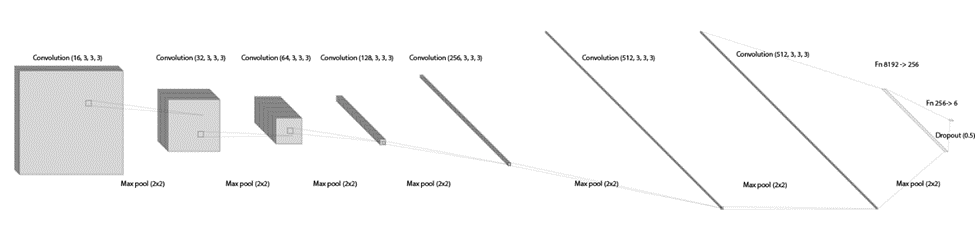
\includegraphics[width=\textwidth]{cnn.png}
    \caption{CNN modelio architektūra}
    \label{fig1}
\end{figure*}

\begin{figure*}[p] 
    \centering
    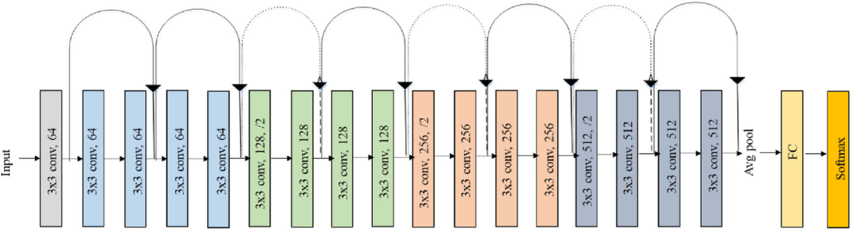
\includegraphics[width=\textwidth]{resnet.png}
    \caption{ResNet-18 modelio architektūra}
    \label{fig2}
\end{figure*}

\begin{figure*}[p]
    \centering
    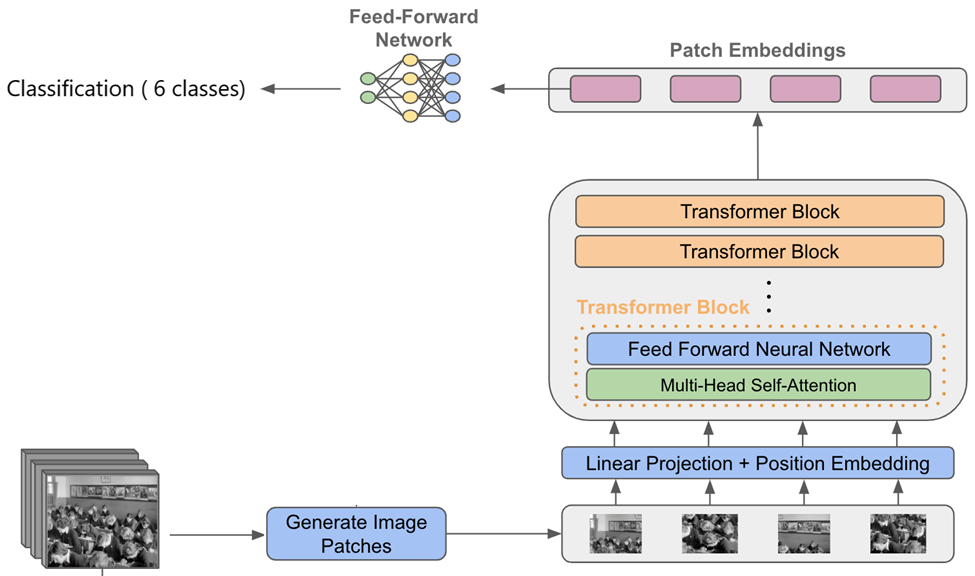
\includegraphics[width=0.7\textwidth]{vit.png}
    \caption{ViT modelio architektūra}
    \label{fig3}
\end{figure*}

\subsection{Metrikų lentelės}

\ref{tab:results2} lent. - CNN 

\ref{tab:results3} lent. - ResNet-18 

\ref{tab:results5} lent. - ViT 

\begin{table*}[p]
    \centering
    \caption{CNN modelio rezultatų metrikų lentelė}
    \label{tab:results2}
    \begin{tabular}{lcccc}
    \hline
    Kategorija & Tikslumas & Precizija & Atkūrimas & F1 balas \\
    \hline
    Financial reports & 0.8413 & 0.7562 & 0.8538 & 0.8029 \\
    Government tenders & 0.8125 & 0.7102 & 0.7719 & 0.7401 \\
    Laws and regulations & 0.7344 & 0.7333 & 0.4624 & 0.5661 \\
    Manuals & 0.7219 & 0.6735 & 0.5489 & 0.6049 \\
    Patents & 0.9471 & 0.9149 & 0.9923 & 0.9513 \\
    Scientific articles & 0.9419 & 0.8655 & 0.9677 & 0.9137 \\
    \hline
    \end{tabular}
\end{table*}

\begin{table*}[p]
    \vfill
    \centering
    \caption{Resnet-18 modelio rezultatų metrikų lentelė}
    \label{tab:results3}
    \begin{tabular}{lcccc}
    \hline
    Kategorija & Tikslumas & Precizija & Atkūrimas & F1 balas \\
    \hline
    Financial reports & 0.8983 & 0.8841 & 0.9474 & 0.9149 \\
    Government tenders & 0.9342 & 0.8889 & 0.8725 & 0.8806 \\
    Laws and regulations & 0.8825 & 0.8846 & 0.8172 & 0.8496 \\
    Manuals & 0.8764 & 0.8644 & 0.7814 & 0.8203 \\
    Patents & 0.9615 & 0.9306 & 0.9654 & 0.9477 \\
    Scientific articles & 0.9801 & 0.9397 & 0.9851 & 0.962 \\
    \hline
    \end{tabular}
\end{table*}

\begin{table*}[p]
    \vfill
    \centering
    \caption{ViT modelio rezultatų metrikų lentelė}
    \label{tab:results5}
    \begin{tabular}{lcccc}
    \hline
    Kategorija & Tikslumas & Precizija & Atkūrimas & F1 balas \\
    \hline
    Financial reports & 0.8123 & 0.7455 & 0.9524 & 0.8358 \\
    Government tenders & 0.7876 & 0.729 & 0.8701 & 0.7938 \\
    Laws and regulations & 0.7016 & 0.6301 & 0.4624 & 0.5336 \\
    Manuals & 0.7406 & 0.6391 & 0.5783 & 0.6074 \\
    Patents & 0.9649 & 0.9565 & 0.9939 & 0.9748 \\
    Scientific articles & 0.9652 & 0.9524 & 0.9641 & 0.9582 \\
    \hline
    \end{tabular}
\end{table*}

\subsection{Klasifikavimo lentelės}

\ref{tab:results1} lent. - CNN 

\ref{tab:results4} lent. - ResNet-18 

\ref{tab:results6} lent. - ViT 

\begin{table*}[p]
    \vfill
    \centering
    \caption{CNN modelio klasifikavimo lentelė}
    \label{tab:results1}
    \resizebox{\textwidth}{!}{
    \begin{tabular}{|l|c|c|c|c|c|c|}
    \hline
    & \multicolumn{6}{c|}{\makecell{Predicted Class}} \\
    \cline{2-7}
    \makecell{Actual\\Class} & Financial reports & Government tenders & Laws and regulations & Manuals & Patents & Scientific articles \\
    \hline
    Financial reports & 151 & 1 & 6 & 11 & 5 & 1\\
    Government tenders & 0 & 88 & 16 & 4 & 0 & 0\\
    Laws and regulations & 2 & 16 & 143 & 8 & 26 & 0\\
    Manuals & 7 & 8 & 21 & 108 & 10 & 6\\
    Patents & 2 & 0 & 7 & 0 & 120 & 1\\
    Scientific articles & 1 & 0 & 1 & 0 & 4 & 129\\
    \hline
    \end{tabular}
    }
\end{table*}

\begin{table*}[p]
    \vfill
    \centering
    \caption{Resnet-18 modelio klasifikavimo lentelė}
    \label{tab:results4}
    \resizebox{\textwidth}{!}{%
    \begin{tabular}{|l|c|c|c|c|c|c|}
    \hline
    & \multicolumn{6}{c|}{\makecell{Predicted Class}} \\
    \cline{2-7}
    \makecell{Actual\\Class} & Financial reports & Government tenders & Laws and regulations & Manuals & Patents & Scientific articles \\
    \hline
    Financial reports & 168 & 1 & 4 & 2 & 0 & 0\\
    Government tenders & 1 & 98 & 4 & 5 & 0 & 0\\
    Laws and regulations & 16 & 7 & 162 & 7 & 3 & 0\\
    Manuals & 17 & 1 & 3 & 129 & 3 & 7\\
    Patents & 0 & 1 & 0 & 2 & 127 & 0\\
    Scientific articles & 1 & 0 & 0 & 1 & 6 & 133\\
    \hline
    \end{tabular}%
    }
\end{table*}

\begin{table*}[p]
    \vfill
    \centering
    \caption{ViT modelio klasifikavimo lentelė}
    \label{tab:results6}
    \resizebox{\textwidth}{!}{%
    \begin{tabular}{|l|c|c|c|c|c|c|}
    \hline
    & \multicolumn{6}{c|}{\makecell{Predicted Class}} \\
    \cline{2-7}
    \makecell{Actual\\Class} & Financial reports & Government tenders & Laws and regulations & Manuals & Patents & Scientific articles \\
    \hline
    Financial reports & 146 & 2 & 3 & 20 & 2 & 2\\
    Government tenders & 0 & 82 & 7 & 19 & 0 & 0\\
    Laws and regulations & 3 & 1 & 118 & 35 & 37 & 1\\
    Manuals & 3 & 2 & 7 & 139 & 7 & 2\\
    Patents & 0 & 0 & 4 & 0 & 125 & 1\\
    Scientific articles & 1 & 0 & 0 & 3 & 3 & 128\\
    \hline
    \end{tabular}%
    }
\end{table*}

\subsection{t-SNE projekcijų pasiskirstymas}

\ref{fig4} pav. - CNN 

\ref{fig5} pav. - ResNet-18 

\ref{fig6} pav. - ViT 

\begin{figure*}[p]
    \vfill
    \centering
    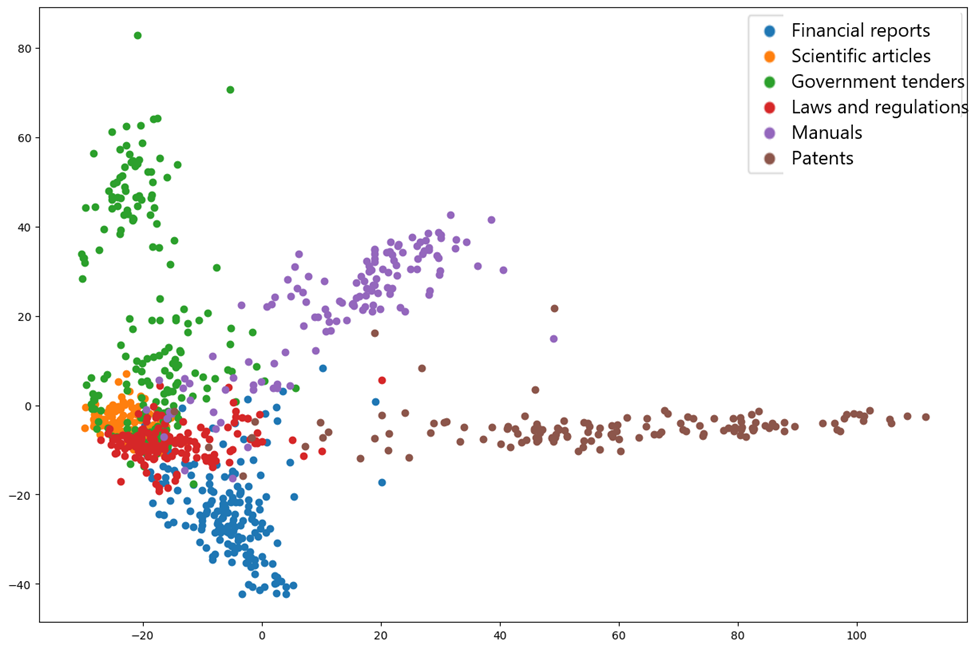
\includegraphics[width=0.6\textwidth]{cnnT2.png}
    \caption{CNN modelio klasių t-SNE projekcijų pasiskirstymas 2-d erdvėje}
    \label{fig4}
\end{figure*}

\begin{figure*}[p]
    \vfill
    \centering
    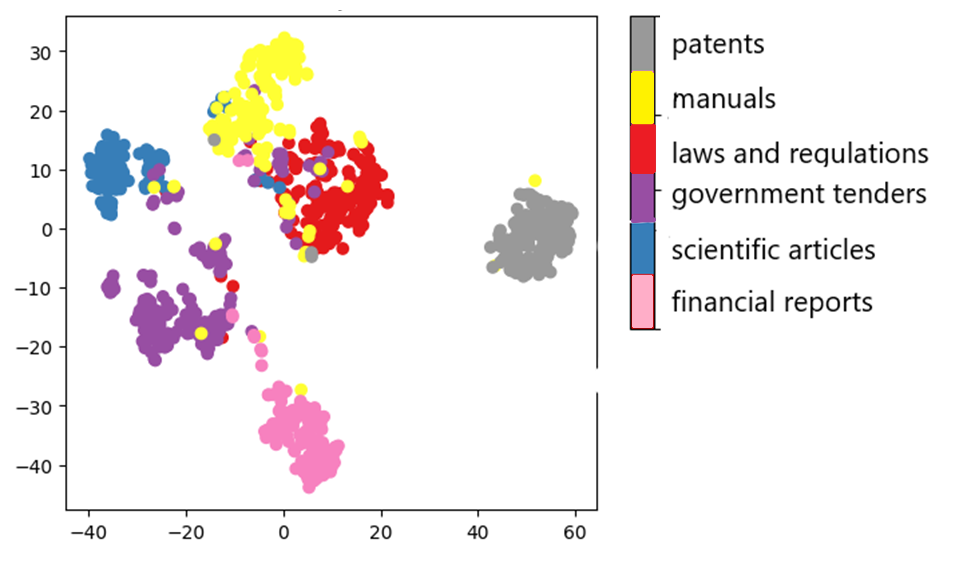
\includegraphics[width=0.6\textwidth]{resnetT1.png}
    \caption{ResNet18 modelio klasių t-SNE projekcijų pasiskirstymas 2-d erdvėje}
    \label{fig5}
\end{figure*}

\begin{figure*}[p]
    \vfill
    \centering
    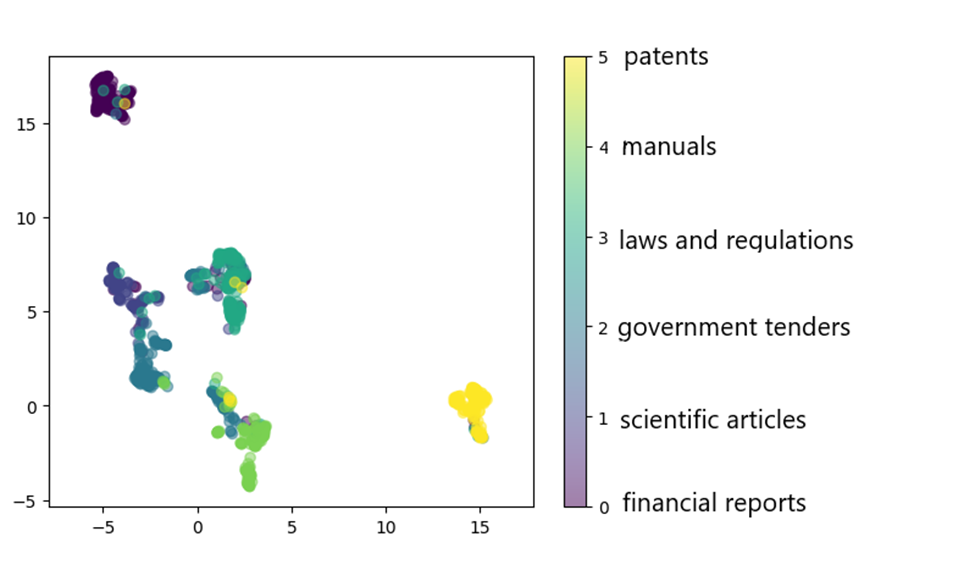
\includegraphics[width=0.6\textwidth]{vitT1.png}
    \caption{ViT modelio klasių t-SNE projekcijų pasiskirstymas 2-d erdvėje}
    \label{fig6}
\end{figure*}

\subsection{Modelių lyginimas}

\ref{tab:comparison} lent.

\begin{table*}[p]
    \vfill
    \centering
    \caption{Modelių lyginimo rezultatai}
    \label{tab:comparison}
    \begin{tabular}{lccc}
    \hline
    Modelis & Testavimo laikas (sekundės) & Parametrų skaičius & Tikslumas \\
    \hline
    CNN (sukurtas) & 18.12 & 6,034,566 & 0.82 \\
    ResNet18 & 20.53 & 11,179,590 & 0.9 \\
    ViT & 25.65 & 85,651,206 & 0.82 \\
    \hline
    \end{tabular}
\end{table*}

\begingroup
\small
\bibliographystyle{unsrtnat}
\bibliography{saltiniai}
\endgroup
\end{document}
